
\section{Experiments}
\begin{frame}
  \frametitle{Hardware}

  \begin{block}{CPU cluster}
    Each node has a: \ttfamily{Intel(R) Xeon(R) Platinum 9242 CPU \@2.30Ghz \\
    with $96$ CPU(s)}, $4$ Non-unified Memory Access (NUMA) nodes and 35.75MB L3 cache.
  \end{block}
  \begin{figure}[htbp]
    \centering
    \begin{tikzpicture}[scale=0.6, transform shape]
      % \node[anchor=south west,inner sep=0] (image) at (0,0) {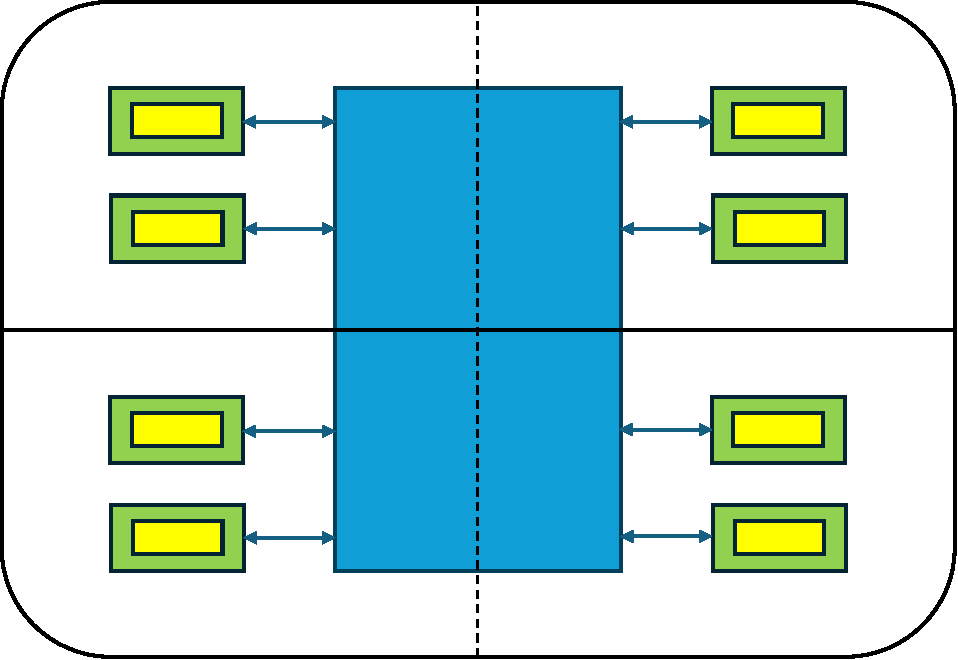
\includegraphics[width=0.5\textwidth]{figure/FIG_Topology_9242.pdf}};
      \node[anchor=south west,inner sep=0] (image) at (0,0) {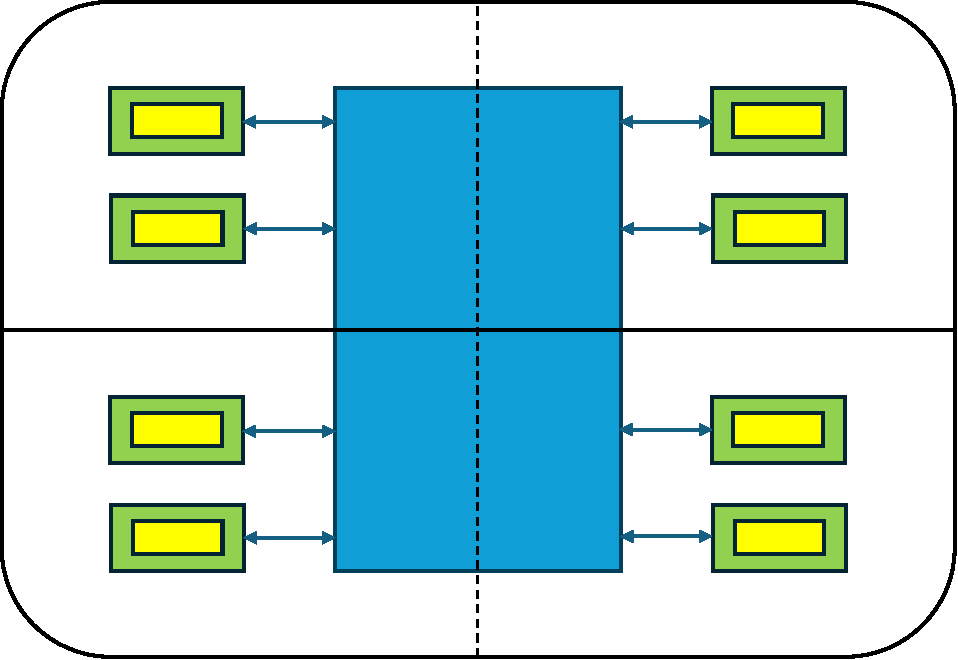
\includegraphics[width=0.56\textwidth]{figure/FIG_Topology_9242.pdf}};     /// overleaf
      \begin{scope}[x={(image.south east)},y={(image.north west)}]
          % \draw[help lines, step=1em] (-1em,-1em) grid (30em,20em);    
          % % Draw axes
          % \draw[dashed,->] (-1em,0) -- (30em,0) node[right] {x};
          % \draw[dashed,->] (0,-1em) -- (0,20em) node[above] {y};
  
        \node at (12em,18em) {$2$ $Scokets$};
  
        \node at (4.5em,1em) {$DDR4$};
        \node at (19.5em,1em) {$DDR4$};
  
        \node at (4.5em, 15em) {$DDR4$};
        \node at (19.5em,15em) {$DDR4$};
  
        \node at (12em,13em) {Hyper-threads};
        \node at (12em,5.5em) {Hyper-threads};
  
        \node at (12em,11em) {$48$ $CPUS$};
        \node at (12em,3.5em) {$48$ $CPUS$};
      \end{scope}
    \end{tikzpicture}
    \caption{NUMA topology of single node on Cluster}
    \label{FIG_Topology_Callan}
  \end{figure}

\end{frame}


\begin{frame}
  \frametitle{Hardware}
  \begin{block}{GPU cluster}
    Each node has a
    \begin{itemize}
      \item AMD Ryzen 7, 7800 X3D, with 16 CPU(s)
      \item NVIDIA RTX 4090, 24GB
    \end{itemize}
  \end{block}

\end{frame}

\subsection{On Single Node}
\begin{frame}
  \frametitle{Single Node Scaling Tests}
  2D Heat Equation\\
  Single Precision \\
  Problem Size: $512^2, 1024^2, 2048^2, 4096^2, 8192^2, 16384^2, 32768^2$ \\




\end{frame}


\begin{frame}
  \frametitle{Single Node Scaling Tests}
  \framesubtitle{Strong Scaling - Pure MPI}
  \begin{figure}[htbp]
    \centering
    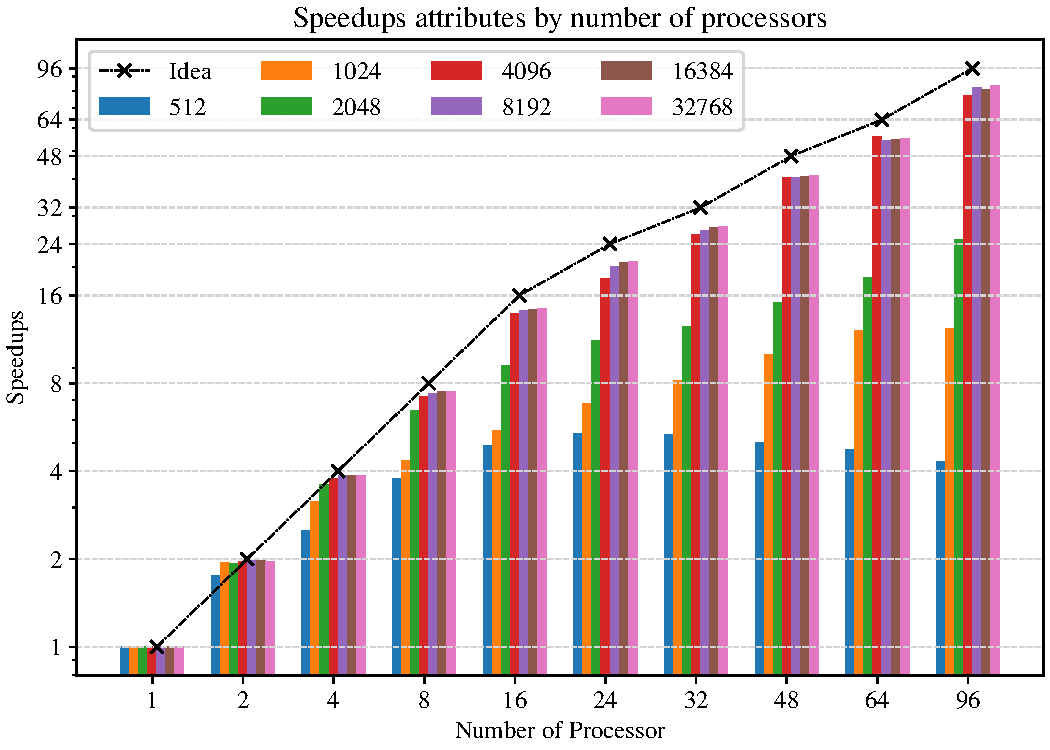
\includegraphics[width=0.56\textwidth]{figure/FIG_Benchmark_pure_mpi.pdf}
    \label{FIG:Benchmark:PURE_MPI}
  \end{figure}
\end{frame}



\begin{frame}
  \frametitle{Single Node Scaling Tests}
  \framesubtitle{Strong Scaling - MPI/OpenMP Hybrid}
  \begin{figure}
    \centering
    \begin{subfigure}{0.41\textwidth}
      \centering
      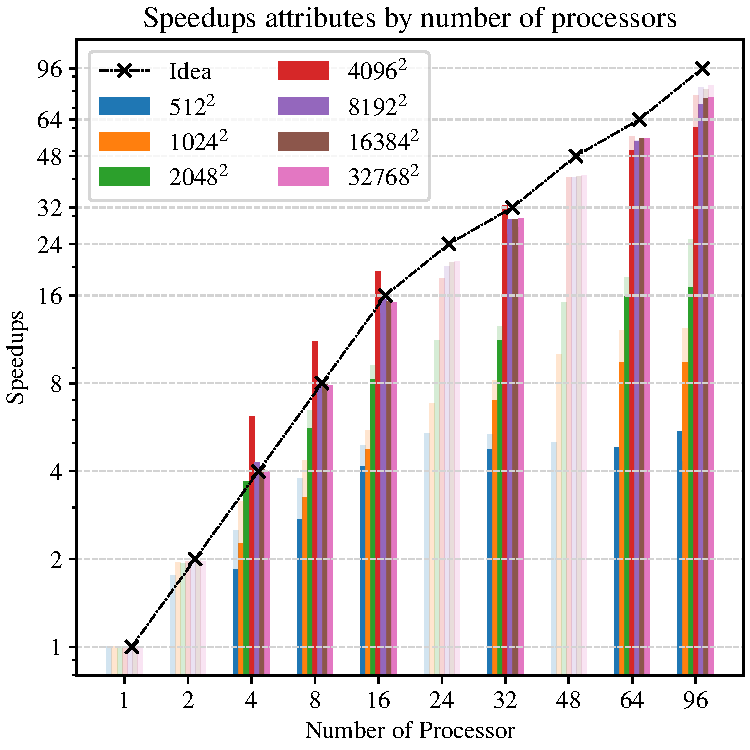
\includegraphics[width=\textwidth]{figure/FIG_Benchmark_hybrid_0.pdf}
      \caption{No overlapping comm./comp.}
      \label{FIG:Benchmark:Hybrid_0}
    \end{subfigure}
    % \hfill
    \begin{subfigure}{0.41\textwidth}
      \centering
      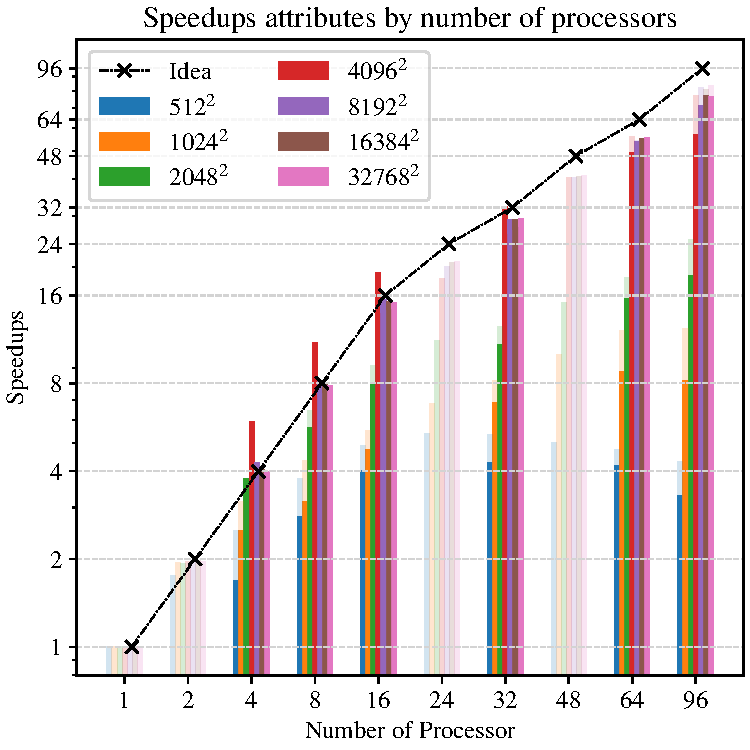
\includegraphics[width=\textwidth]{figure/FIG_Benchmark_hybrid_1.pdf}
      \caption{With overlapping comm./comp.}
      \label{FIG:Benchmark:Hybrid_1}
    \end{subfigure}
    % \caption{
    %   Comparison of speedup ratios of strong scaling tests of master-only parallelized program with overlapping and no overlapping of computation and communication.  
    %   The vague background is the results of pure MPI parallelization from Figure \ref{FIG:Benchmark:PURE_MPI}, and the problem scales are identical as well.
    %   The number of threads are set to $1$, $2$, $4$, $8$, $16$, and $24$, 
    %   tasks per CPU are $1$, $2$ and $4$.
    % }
    \label{FIG:Benchmark:Hybrid}
  \end{figure}
\end{frame}

\begin{frame}
  \frametitle{Single Node Scaling Tests}
  \framesubtitle{Weak Scaling}

  \begin{center}
    % \captionof{table}{Weak Scaling on Single Node of 2D Heat Equation}  % Use captionof to replace table environment
    \label{TAB:Benchmark:Weak_PURE_MPI}
    \footnotesize
    \begin{tabular}{p{3cm} p{1.5cm} p{1.5cm} p{1.5cm} p{1.5cm} p{1cm}}
      \toprule
      \multirow{2}{*}{\bfseries Strategy}     & \multirow{2}{*}{\bfseries Size} & \multicolumn{3}{c}{\bfseries Number of CPUs}   & \multirow{2}{*}{\bfseries $f_p(\%)$}  \\
                                    &                                  & \bfseries 4   & \bfseries 16   & \bfseries 64  &                                       \\
      \midrule
      \bfseries Pure MPI      & \multirow{3}{*}{$512^2$}      & 4.006  & 12.497  & 47.849                                         & 75.1 \\
      \bfseries No Overlap    &                               & 2.876  & 11.206  & 42.754                                         & 67.0 \\
      \bfseries With Overlap  &                               & 3.173  & 10.818  & 42.282                                         & 66.2 \\
      \midrule
      \bfseries Pure MPI      & \multirow{3}{*}{$1024^2$}     & 3.838  & 9.304   & 33.707                                         & 53.2  \\
      \bfseries No Overlap    &                               & 3.947  & 12.995  & 33.447                                         & 54.1 \\
      \bfseries With Overlap  &                               & 4.024  & 12.932  & 33.361                                         &  54.0 \\
      \midrule
      \bfseries Pure MPI      & \multirow{3}{*}{$2048^2$}     & 2.376  & 8.245   & 31.203                                         &  49.0\\
      \bfseries No Overlap    &                               & 3.874  & 8.972   & 31.510                                         &  49.8 \\
      \bfseries With Overlap  &                               & 3.740  & 8.989   & 31.430                                         &  49.7 \\
      \midrule
      \bfseries Pure MPI      & \multirow{3}{*}{$4096^2$}     & 3.543  & 8.245   & 31.203                                         &  77.5\\
      \bfseries No Overlap    &                               & 3.953  & 13.799  & 49.515                                         &  78.0\\
      \bfseries With Overlap  &                               & 3.948  & 13.800  & 49.989                                         &  78.7 \\
      \bottomrule
    \end{tabular}
  \end{center}
\end{frame}









\subsection{On Multi-node}
\begin{frame}
  \frametitle{Multi-node Scaling Tests}
  \framesubtitle{Strong Scaling - Pure MPI}

  \begin{figure}[htbp]
    \centering
    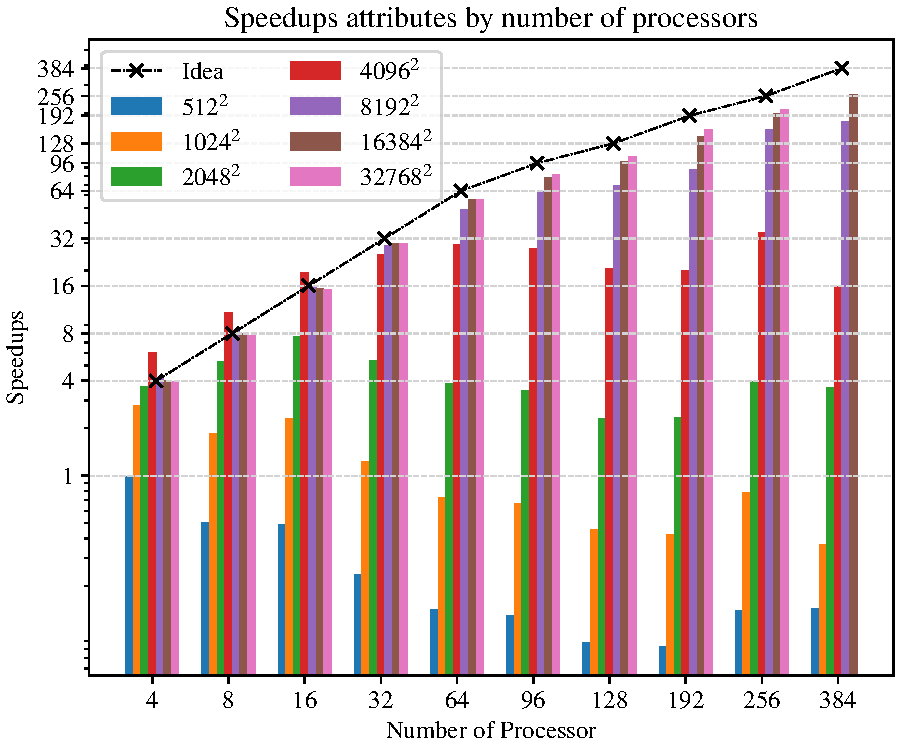
\includegraphics[width=0.55\textwidth]{figure/FIG_Benchmark_pure_mpi_multi_nodes.pdf}
    \caption{
      Comparison of speedup ratios of strong scaling tests of pure MPI parallelized program. 
      The investigated problem scales are the power of $2$, exponents ranging from $9$ to $15$.
      The number of CPUs are also set as power of $2$, with additional numbers $96$, $192$ and $384$ matched the topologies of CPU.
    }
    \label{FIG:Benchmark:PURE_MPI_Multi_Node}
  \end{figure}
\end{frame}



\begin{frame}
  \frametitle{Multi-node Scaling Tests}
  \framesubtitle{Strong Scaling - MPI/OpenMP Hybrid}
  \begin{figure}
    \centering
    \begin{subfigure}{0.47\textwidth}
      \centering
      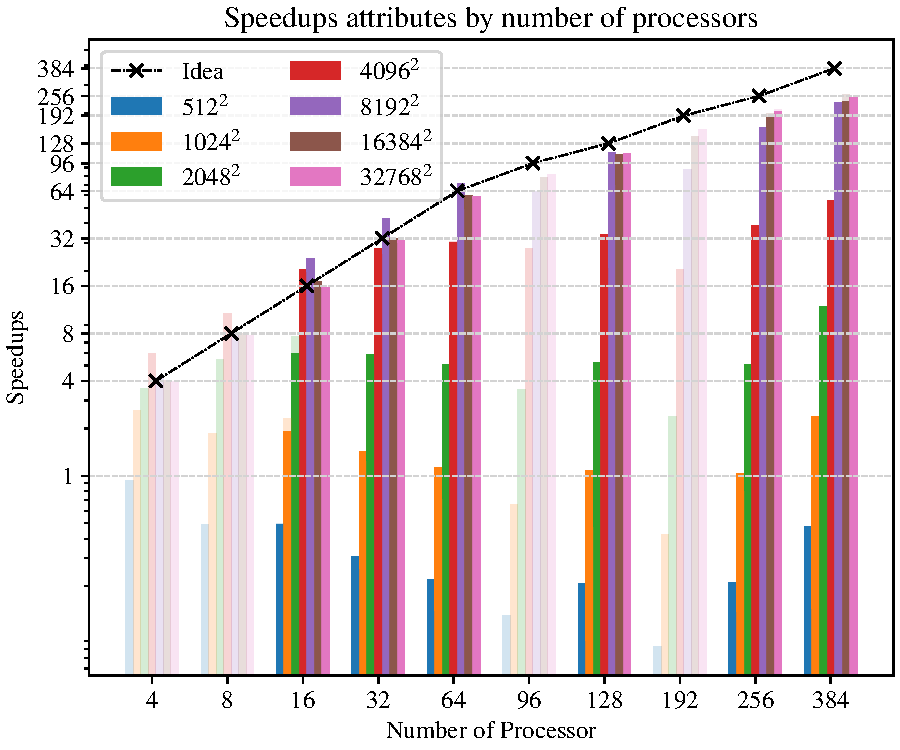
\includegraphics[width=\textwidth]{figure/FIG_Benchmark_hybrid_0_multi_nodes.pdf}
      \caption{No overlapping comm./comp.}
      \label{FIG:Benchmark:Hybrid_0_Multi_Node}
    \end{subfigure}
    % \hfill
    \begin{subfigure}{0.47\textwidth}
      \centering
      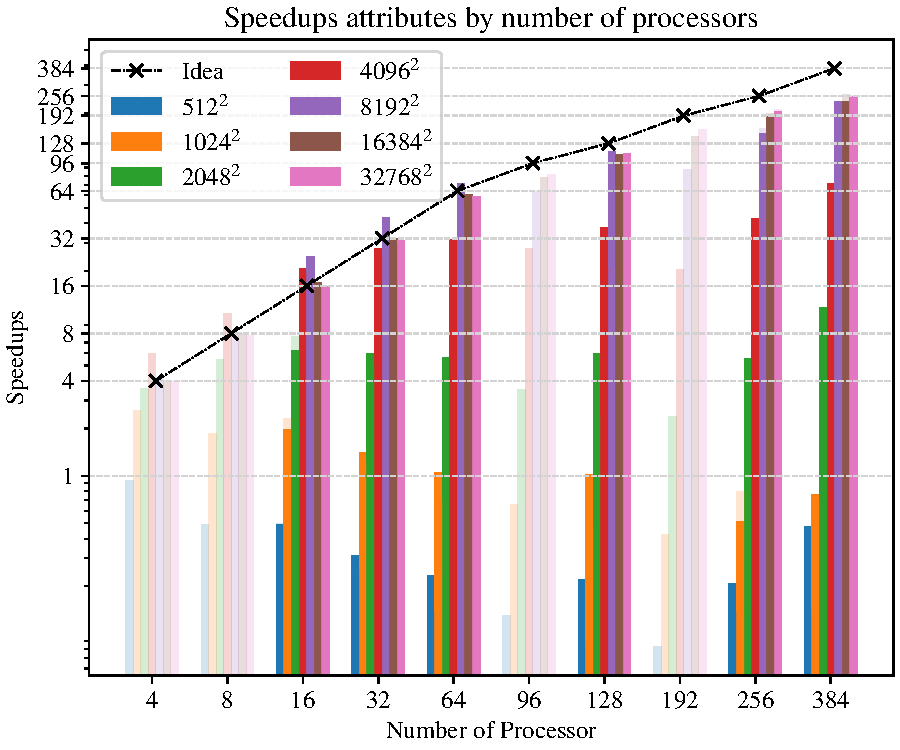
\includegraphics[width=\textwidth]{figure/FIG_Benchmark_hybrid_1_multi_nodes.pdf}
      \caption{With overlapping comm./comp.}
      \label{FIG:Benchmark:Hybrid_1_Multi_Node}
    \end{subfigure}
    % \caption{
      % Comparison of speedup ratios of strong scaling tests on $4$ nodes of 
      % mater-only parallelized program with overlapping and no overlapping of computation and communication.  
      % The vague background is the results of pure MPI parallelization from figure 
      % \ref{FIG:Benchmark:PURE_MPI_Multi_Node} and problems sclaes are identical as well.
      % The number of threads are set to $1$, $2$, $4$, $8$, $16$, and $24$, 
      % tasks per CPU are $1$, $2$ and $4$.
    % }
    \label{FIG:Benchmark:Hybrid_Multi_Node}
  \end{figure}
\end{frame}


\begin{frame}
  \frametitle{Multi-node Scaling Tests}
  \framesubtitle{Weak Scaling}

  % \begin{table}[htbp]
  %   \caption{Weak Scaling on Multi-node of 2D Heat Equation}
  %   \label{TAB:Benchmark:Weak_PURE_MPI_Multi_Node}
  %   \begin{minipage}{\columnwidth}
  %     \begin{center}
  %       \footnotesize % overleaf
  %       \begin{tabular}{>{\bfseries}p{3cm} p{1.5cm} p{1.5cm} p{1.5cm} p{1.5cm} p{1.5cm} p{1cm}}
  %         \toprule
  %         \multirow{2}{*}{Strategy}     & \multirow{2}{*}{\bfseries Size} & \multicolumn{4}{c}{\bfseries  Number of CPUs}   & \multirow{2}{*}{\bfseries $f_p(\%)$}  \\
  %                                       &                                 & \bfseries 4   & \bfseries 16   & \bfseries 64  & \bfseries 256  &                        \\
  %         \midrule
  %         Pure MPI      & \multirow{3}{*}{$512^2$}      & 3.300  & 10.379  & 26.000   & 124.375                                    & 48.2 \\
  %         No Overlap    &                               &   -    &  8.094  & 25.931   & 127.648                                    & 49.3 \\
  %         With Overlap  &                               &   -    &  8.386  & 27.126   & 116.951                                    & 45.5 \\
  %         \midrule
  %         Pure MPI      & \multirow{3}{*}{$1024^2$}     & 3.848  & 13.037  & 30.143   &   -                                        & 49.3 \\
  %         No Overlap    &                               &   -    & 13.702  & 44.040   &   -                                        & 69.8 \\
  %         With Overlap  &                               &   -    & 13.834  & 44.090   &   -                                        & 69.9 \\
  %         \midrule
  %         Pure MPI      & \multirow{3}{*}{$2048^2$}     & 3.787  & 9.172   & 32.013   &   -                                        & 50.6 \\
  %         No Overlap    &                               &   -    & 13.936  & 34.368   &   -                                        & 55.7 \\
  %         With Overlap  &                               &   -    & 14.274  & 34.414   &   -                                        & 55.9 \\
  %         \midrule
  %         Pure MPI      & \multirow{3}{*}{$4096^2$}     & 3.884  & 13.859  & 51.041   &   -                                        & 80.2 \\
  %         No Overlap    &                               &   -    & 15.315  & 53.157   &   -                                        & 83.8 \\
  %         With Overlap  &                               &   -    & 15.294  & 53.401   &   -                                        & 84.2 \\
  %         \bottomrule
  %       \end{tabular}
  %     \end{center}
  %     % \bigskip
  %     % \footnotesize\emph{Source:} This is source 
  %   \end{minipage}
  % \end{table}


  \begin{center}
    % \caption{Weak Scaling on Multi-node of 2D Heat Equation}  % Use captionof to replace table environment
    \label{TAB:Benchmark:Weak_PURE_MPI_Multi_Node}
    \footnotesize
    \begin{tabular}{p{3cm} p{1.5cm} p{1.5cm} p{1.5cm} p{1.5cm} p{1.5cm} p{1cm}}
      \toprule
      \multirow{2}{*}{\bfseries Strategy}     & \multirow{2}{*}{\bfseries Size} & \multicolumn{4}{c}{\bfseries  Number of CPUs}   & \multirow{2}{*}{\bfseries $f_p(\%)$}  \\
                                    &                                 & \bfseries 4   & \bfseries 16   & \bfseries 64  & \bfseries 256  &                        \\
      \midrule
      \bfseries Pure MPI      & \multirow{3}{*}{$512^2$}      & 3.300  & 10.379  & 26.000   & 124.375                                    & 48.2 \\
      \bfseries No Overlap    &                               &   -    &  8.094  & 25.931   & 127.648                                    & 49.3 \\
      \bfseries With Overlap  &                               &   -    &  8.386  & 27.126   & 116.951                                    & 45.5 \\
      \midrule
      \bfseries Pure MPI      & \multirow{3}{*}{$1024^2$}     & 3.848  & 13.037  & 30.143   &   -                                        & 49.3 \\
      \bfseries No Overlap    &                               &   -    & 13.702  & 44.040   &   -                                        & 69.8 \\
      \bfseries With Overlap  &                               &   -    & 13.834  & 44.090   &   -                                        & 69.9 \\
      \midrule
      \bfseries Pure MPI      & \multirow{3}{*}{$2048^2$}     & 3.787  & 9.172   & 32.013   &   -                                        & 50.6 \\
      \bfseries No Overlap    &                               &   -    & 13.936  & 34.368   &   -                                        & 55.7 \\
      \bfseries With Overlap  &                               &   -    & 14.274  & 34.414   &   -                                        & 55.9 \\
      \midrule
      \bfseries Pure MPI      & \multirow{3}{*}{$4096^2$}     & 3.884  & 13.859  & 51.041   &   -                                        & 80.2 \\
      \bfseries No Overlap    &                               &   -    & 15.315  & 53.157   &   -                                        & 83.8 \\
      \bfseries With Overlap  &                               &   -    & 15.294  & 53.401   &   -                                        & 84.2 \\
      \bottomrule
    \end{tabular}
  \end{center}
\end{frame}


\subsection{On Different Dimensions}
\begin{frame}
  \frametitle{3D Space Heat Equation}
  \framesubtitle{Strong Scaling - pure MPI}
  
  \begin{figure}
    \centering
    \begin{subfigure}{0.42\textwidth}
      \centering
      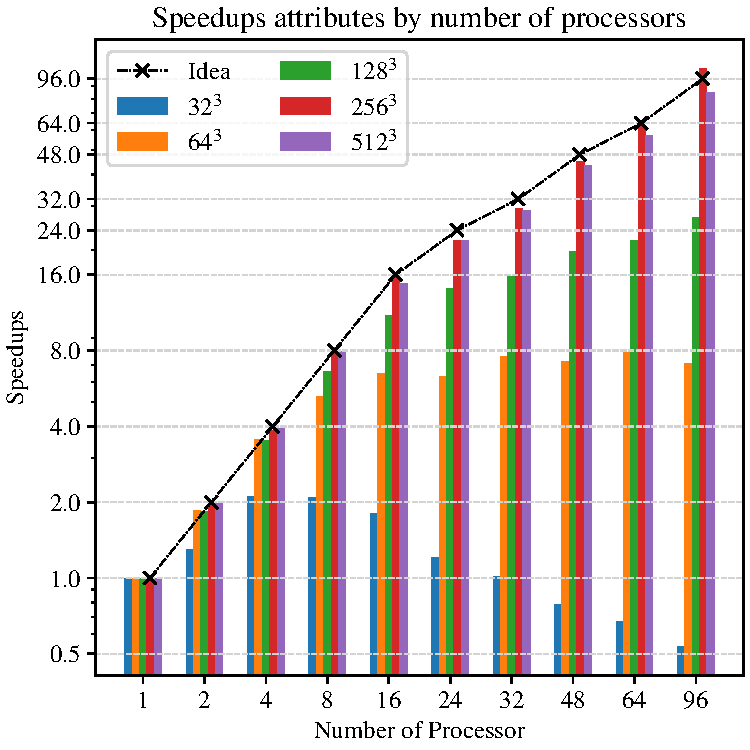
\includegraphics[width=\textwidth]{figure/FIG_Benchmark_pure_mpi_3D.pdf}
      \caption{Single node}
      \label{FIG:Benchmark:Pure_MPI_Single_Node_3D}
    \end{subfigure}
    % \hfill
    \begin{subfigure}{0.42\textwidth}
      \centering
      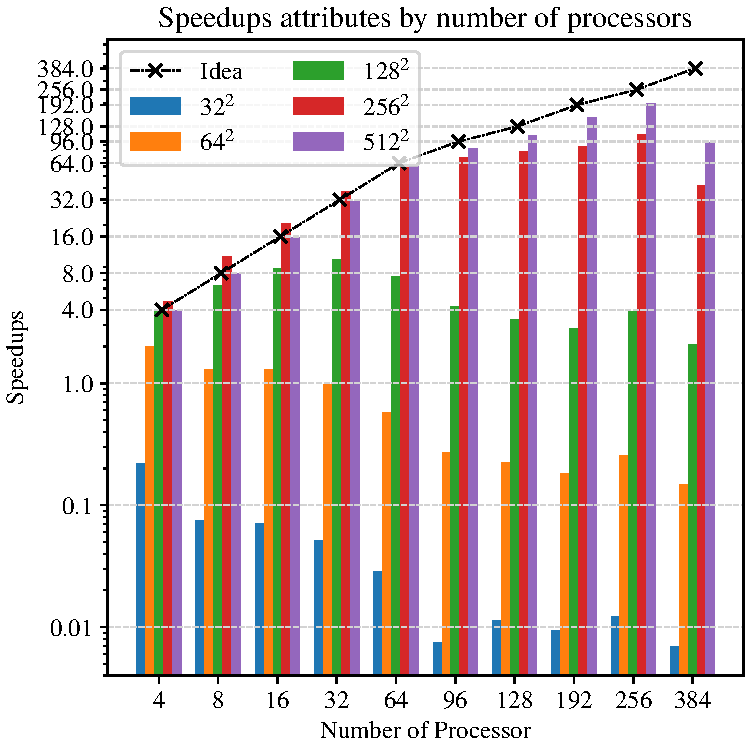
\includegraphics[width=\textwidth]{figure/FIG_Benchmark_pure_mpi_3D_multi_nodes.pdf}
      \caption{Four nodes}
      \label{FIG:Benchmark:Pure_MPI_Multi_Node_3D}
    \end{subfigure}
    % \caption{
      % Comparison of speedup ratios of strong scaling tests  pure MPI models on $4$ nodes of and $1$ node.
      % The problem sizes are set to $32^3$, $64^3$, $128^3$, $256^3$ and $512^3$ with single precision.
    % }
    \label{FIG:Benchmark:Pure_MPI_Node_3D}
  \end{figure}
  
\end{frame}



\begin{frame}
  \frametitle{3D Space Heat Equation}
  \framesubtitle{Strong Scaling - MPI/OpenMP Hybrid, Single Node}



  \begin{figure}
    \centering
    \begin{subfigure}{0.42\textwidth}
      \centering
      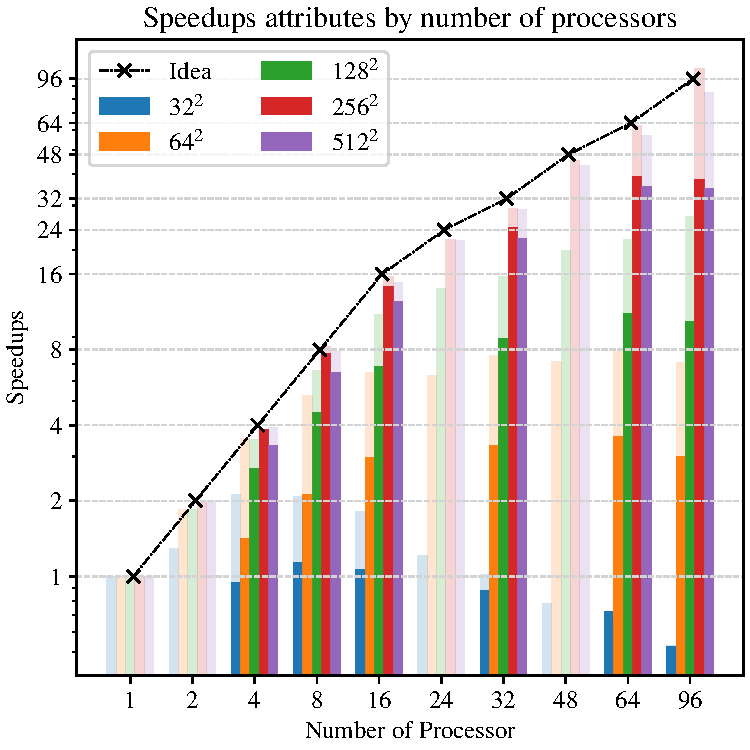
\includegraphics[width=\textwidth]{figure/FIG_Benchmark_hybrid_0_single_nodes_3D.pdf}
      \caption{Non-overlapping}
      \label{FIG:Benchmark:FIG_Benchmark_hybrid_0_single_nodes_3D}      
    \end{subfigure}
    % \hfill
    \begin{subfigure}{0.42\textwidth}
      \centering
      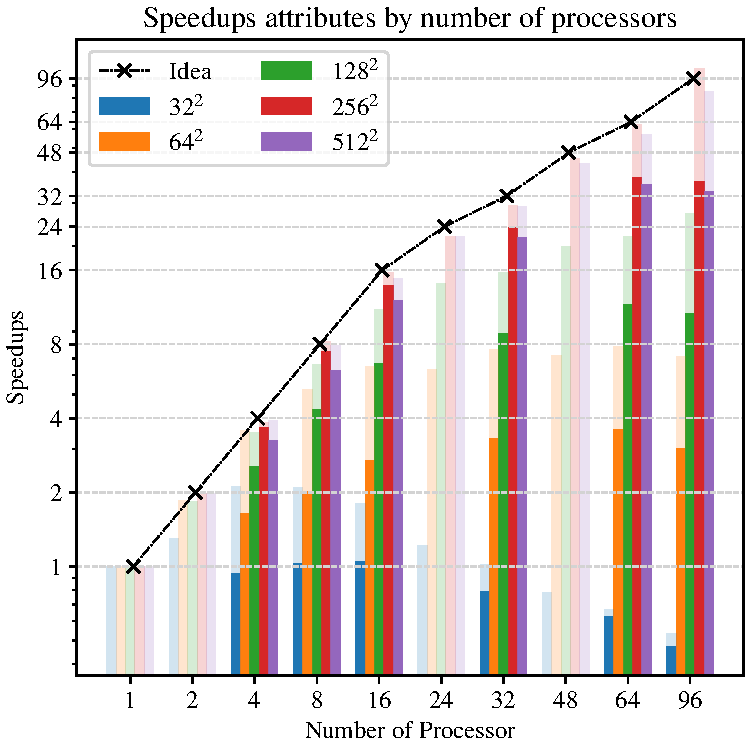
\includegraphics[width=\textwidth]{figure/FIG_Benchmark_hybrid_1_single_nodes_3D.pdf}
      \caption{With overlapping}
      \label{FIG:Benchmark:FIG_Benchmark_hybrid_1_single_nodes_3D}
    \end{subfigure}
    % \caption{
      % Comparison of speedup ratios of strong scaling tests  pure MPI models on $4$ nodes of and $1$ node.
      % The problem sizes are set to $32^3$, $64^3$, $128^3$, $256^3$ and $512^3$ with single precision.
    % }
    \label{FIG:Benchmark:Hybrid_Single_Node_3D}
  \end{figure}

\end{frame}






% \begin{figure}[htbp]
%   \centering
%   \subfigure[Single Node, Non-overlapping]{
%     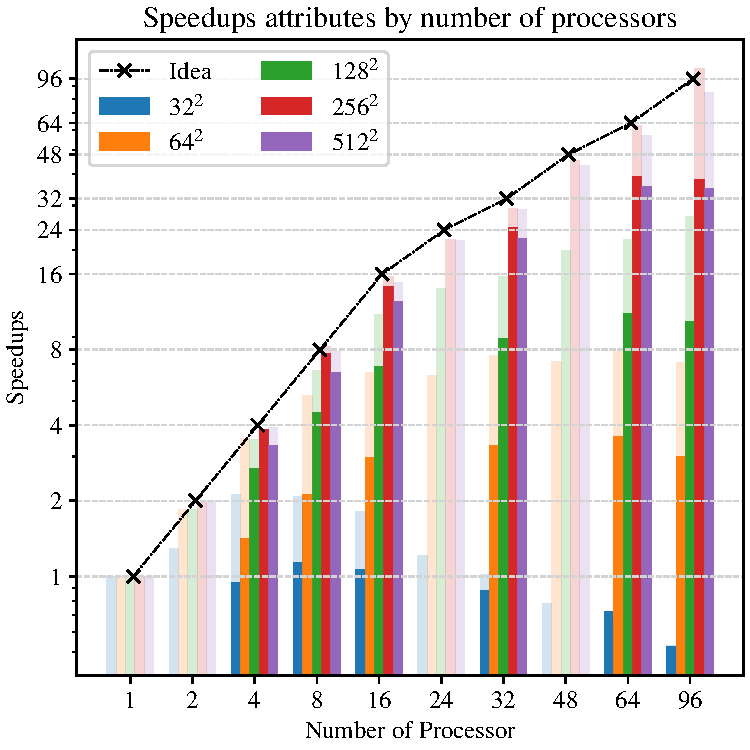
\includegraphics[width=0.38\textwidth]{figure/FIG_Benchmark_hybrid_0_single_nodes_3D.pdf}
%     \label{FIG:Benchmark:FIG_Benchmark_hybrid_0_single_nodes_3D}
%   }
%   \hspace{0em} 
%   \subfigure[Single Node, With overlapping]{
%     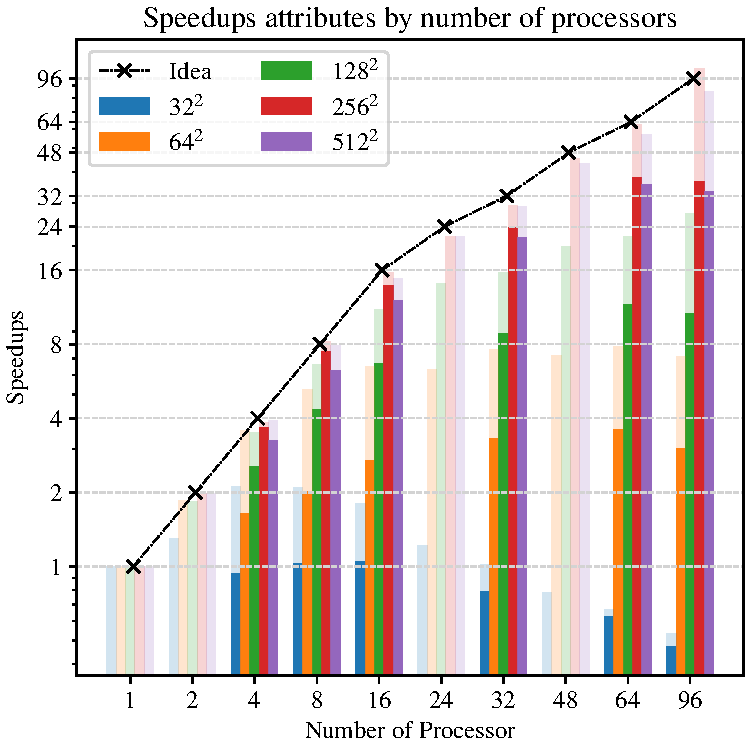
\includegraphics[width=0.38\textwidth]{figure/FIG_Benchmark_hybrid_1_single_nodes_3D.pdf}
%     \label{FIG:Benchmark:FIG_Benchmark_hybrid_1_single_nodes_3D}
%   }
%   \hspace{0em} 
%   \subfigure[Multi-node, Non-overlapping]{
%     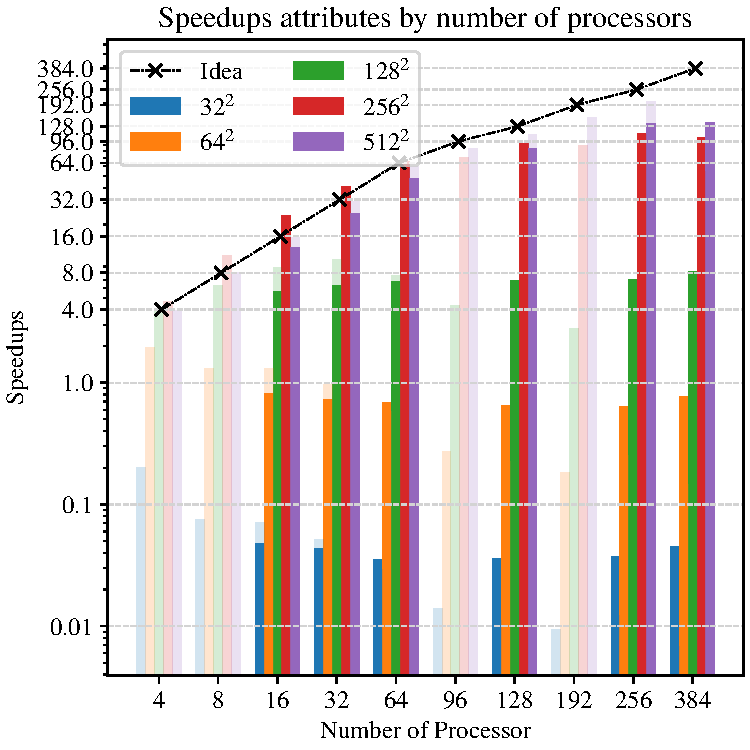
\includegraphics[width=0.38\textwidth]{figure/FIG_Benchmark_hybrid_0_multi_nodes_3D.pdf}
%     \label{FIG:Benchmark:FIG_Benchmark_hybrid_0_multi_nodes_3D}
%   }
%   \hspace{0em} 
%   \subfigure[Multi-node, With overlapping]{
%     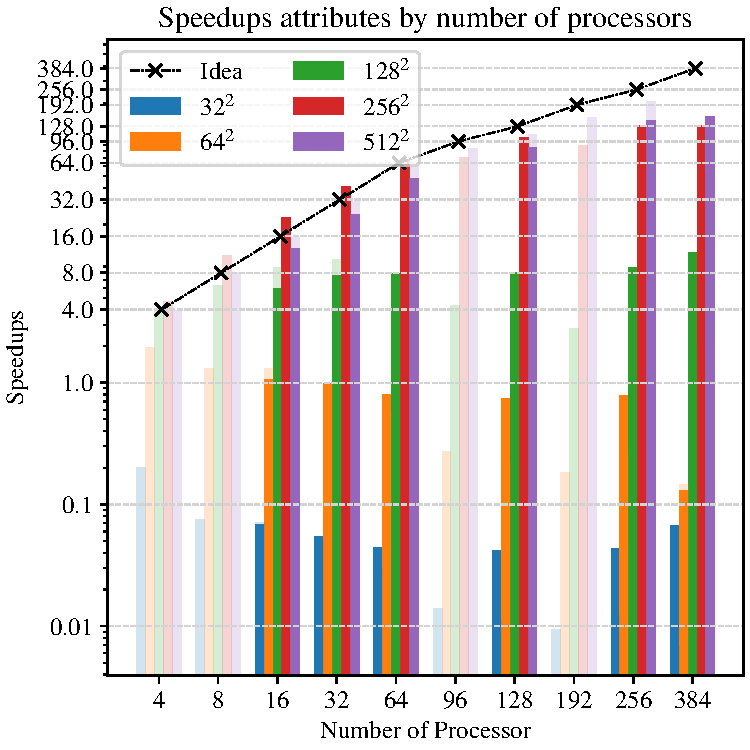
\includegraphics[width=0.38\textwidth]{figure/FIG_Benchmark_hybrid_1_multi_nodes_3D.pdf}
%     \label{FIG:Benchmark:FIG_Benchmark_hybrid_1_multi_nodes_3D}
%   }
%   \caption{
%       Comparison of strong scaling speedup ratios of hybrid models on $4$ compute nodes for solving 3D heat euqations.
%       The problem scales are set to the cude of $32$, $64$, $128$, $256$ and $512$ with single precision.
%       The value background is the strong scaling results of figure \ref{FIG:Benchmark:Pure_MPI_Node_3D}.
%     }
%   \label{FIG:Benchmark:Hybrid_Single_Four_Node_3D}
% \end{figure}



\begin{frame}
  \frametitle{3D Space Heat Equation}
  \framesubtitle{Strong Scaling - MPI/OpenMP Hybrid, Four Nodes}
  

  
  \begin{figure}
    \centering
    \begin{subfigure}{0.42\textwidth}
      \centering
      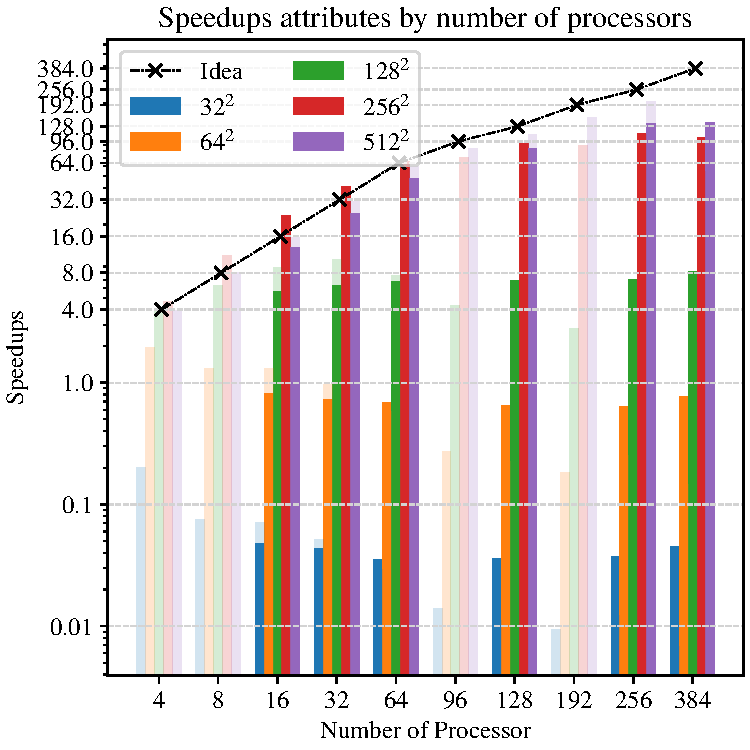
\includegraphics[width=\textwidth]{figure/FIG_Benchmark_hybrid_0_multi_nodes_3D.pdf}
      \caption{Non-overlapping}
      \label{FIG:Benchmark:FIG_Benchmark_hybrid_0_multi_nodes_3D}
    \end{subfigure}
    % \hfill
    \begin{subfigure}{0.42\textwidth}
      \centering
      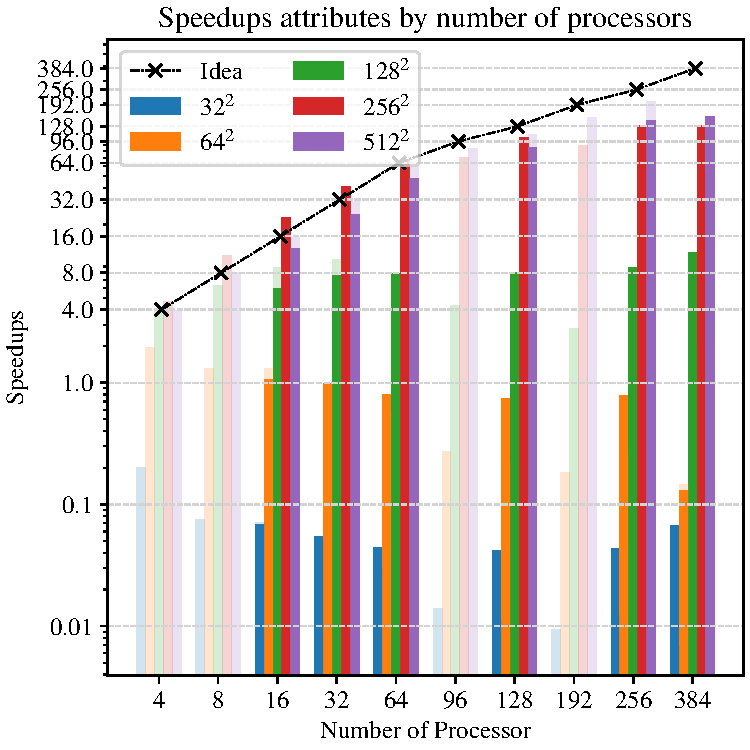
\includegraphics[width=\textwidth]{figure/FIG_Benchmark_hybrid_1_multi_nodes_3D.pdf}
      \caption{With overlapping}
      \label{FIG:Benchmark:FIG_Benchmark_hybrid_1_multi_nodes_3D}
    \end{subfigure}
    % \caption{
      % Comparison of speedup ratios of strong scaling tests  pure MPI models on $4$ nodes of and $1$ node.
      % The problem sizes are set to $32^3$, $64^3$, $128^3$, $256^3$ and $512^3$ with single precision.
    % }
    \label{FIG:Benchmark:Hybrid_Four_Node_3D}
  \end{figure}

  
\end{frame}



\begin{frame}
  \frametitle{3D Space Heat Equation}
  \framesubtitle{Weak Scaling}


  % \begin{table}[htbp]
    % \caption{Weak Scaling of 3D Heat Equation}
  %   \label{TAB:Benchmark:Weak_3D_AllModels}
  %   \begin{minipage}{\columnwidth}
      \begin{center}
        \footnotesize % overleaf
        \begin{tabular}{p{2.5cm} p{1cm} p{1.5cm} p{1.5cm} p{1.5cm} p{1.5cm} p{1cm} p{1cm}}
          \toprule
          \multirow{2}{*}{\bfseries Strategy} & \multirow{2}{*}{\bfseries Size} & \multicolumn{3}{c}{\bfseries  Number of CPUs}    & \multirow{2}{*}{\bfseries $f_p(\%)$}  & \multirow{2}{*}{\bfseries $f_p(\%)_{\text{Multi-node}}$}\\
                        &                      & \bfseries 8     & \bfseries 64        & \bfseries 64$_{\text{Multi-node}}$   &  &  &         \\
          \midrule
          \bfseries Pure MPI      & \multirow{3}{*}{$32^3$}       & 5.243  & 26.405              &  9.078                     & 41.6 & 14.2 \\
          \bfseries No Overlap    &                               & 2.124  & 13.386              &  8.094                     & 21.0 &  12.7\\
          \bfseries With Overlap  &                               & 2.014  & 13.884              &  9.586                     & 21.8 & 39.7 \\
          \midrule
          \bfseries Pure MPI      & \multirow{3}{*}{$64^3$}       & 7.937  & 32.034              &  30.106                    & 50.8 & 47.1 \\
          \bfseries No Overlap    &                               & 5.393  & 20.007              &  33.460                    & 31.8 & 52.3 \\
          \bfseries With Overlap  &                               & 5.200  & 19.558              &  35.254                    & 31.1 & 31.6 \\
          \midrule
          \bfseries Pure MPI      & \multirow{3}{*}{$128^3$}      & 3.513  & 24.239              &  25.428                    & 38.0 & 39.7 \\
          \bfseries No Overlap    &                               & 3.303  & 15.235              &  35.254                    & 24.1 & 55.1 \\
          \bfseries With Overlap  &                               & 3.187  & 15.107              &  20.096                    & 23.9 & 31.4 \\
          \bottomrule
        \end{tabular}
      \end{center}
      % \bigskip
      % \footnotesize\emph{Source:} This is source 
  %   \end{minipage}
  % \end{table}
  

\end{frame}






\subsection{With PINN on accuracy}


\begin{frame}
  \frametitle{PINN v.s. FDTD}
  \framesubtitle{Accuracy}

  \begin{table}
    \caption{Mean Square Error of Results}
    \begin{center}
      \footnotesize
      \begin{tabular}{p{1.5cm} p{1.5cm} p{1.5cm}}
        \toprule
        \bfseries Method  & \bfseries Heat 2D      & \bfseries Heat 3D         \\
        \midrule 
        \bfseries FDTD    & 1.7287  & 953.84 \\
        \bfseries PINN    & 13.37   & 24.896 \\
        \bottomrule 
        \multicolumn{3}{l}{Tolerance: $10^{-4}$} \\
      \end{tabular}
    \end{center}
  \end{table}


  

\end{frame}

\begin{frame}
  \frametitle{PINN v.s. FDTD}
  \framesubtitle{Memory Usage v.s. Time of Convergence}

  
  \begin{figure}[htbp]
    \centering
    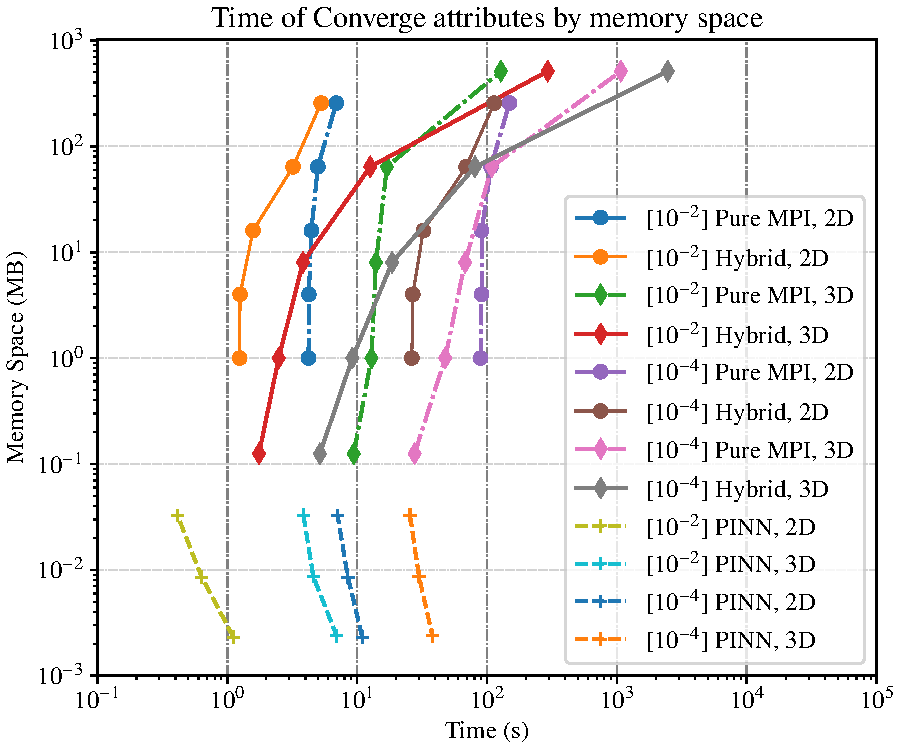
\includegraphics[width=0.45\textwidth]{figure/FIG_Benchmark_Time_Tol.pdf}
    \caption{
      % Comparison of memory usage of FDTD and PINN attributed by time of trainning/converging time consumption for 
      % both 2 dimension and 3 dimension heat equations with single precision. 
      % The predefined tolerance for training and converging are $10^{-2}$ and $10^{-4}$.
      % FDTD was testing on four compute nodes (384 CPUs), and using pure MPI and non-overlapping hybrid models.
      % The PINN models are trained on single NVIDIA RTX 4090 graphics card.
    }
    \label{FIG:Benchmark:TimeTol}
  \end{figure}
\end{frame}

